\documentclass{standalone}

\usepackage[T1]{fontenc}
\usepackage[utf8]{inputenc}
\usepackage{eulervm}
\usepackage{amsmath}
\usepackage{bm}
\usepackage{tikz}
\usepackage{environ}
\usepackage{circuitikz}

\usetikzlibrary{fit}
\usetikzlibrary{patterns}
\usetikzlibrary{arrows}
\usetikzlibrary{positioning}

\usepackage{color}

\definecolor{Comment}{RGB}{97,161,176}

\definecolor{btfGreen}{RGB}{51,160,44}
\definecolor{btfRed}{RGB}{190,60,90}

\definecolor{bleuUni}{RGB}{0, 157, 224}
\definecolor{marronUni}{RGB}{68, 58, 49}
\definecolor{grayMarronUni}{RGB}{60, 60, 60}
\definecolor{grayBleuUni}{RGB}{118, 118, 118}

\definecolor{bluecite}{HTML}{009DE0}

\definecolor{Paired-2}{RGB}{166,206,227}
\definecolor{Paired-1}{RGB}{31,120,180}
\definecolor{Paired-4}{RGB}{178,223,138}
\definecolor{Paired-3}{RGB}{51,160,44}
\definecolor{Paired-6}{RGB}{251,154,153}
\definecolor{Paired-5}{RGB}{227,26,28}
\definecolor{Paired-8}{RGB}{253,191,111}
\definecolor{Paired-7}{RGB}{255,127,0}
\definecolor{Paired-10}{RGB}{202,178,214}
\definecolor{Paired-9}{RGB}{106,61,154}
\definecolor{Paired-12}{RGB}{255,255,153}
\definecolor{Paired-11}{RGB}{177,89,40}
\definecolor{Accent-1}{RGB}{127,201,127}
\definecolor{Accent-2}{RGB}{190,174,212}
\definecolor{Accent-3}{RGB}{253,192,134}
\definecolor{Accent-4}{RGB}{255,255,153}
\definecolor{Accent-5}{RGB}{56,108,176}
\definecolor{Accent-6}{RGB}{240,2,127}
\definecolor{Accent-7}{RGB}{191,91,23}
\definecolor{Accent-8}{RGB}{102,102,102}
\definecolor{Spectral-1}{RGB}{158,1,66}
\definecolor{Spectral-2}{RGB}{213,62,79}
\definecolor{Spectral-3}{RGB}{244,109,67}
\definecolor{Spectral-4}{RGB}{253,174,97}
\definecolor{Spectral-5}{RGB}{254,224,139}
\definecolor{Spectral-6}{RGB}{255,255,191}
\definecolor{Spectral-7}{RGB}{230,245,152}
\definecolor{Spectral-8}{RGB}{171,221,164}
\definecolor{Spectral-9}{RGB}{102,194,165}
\definecolor{Spectral-10}{RGB}{50,136,189}
\definecolor{Spectral-11}{RGB}{94,79,162}
\definecolor{Set1-1}{RGB}{228,26,28}
\definecolor{Set1-2}{RGB}{55,126,184}
\definecolor{Set1-3}{RGB}{77,175,74}
\definecolor{Set1-4}{RGB}{152,78,163}
\definecolor{Set1-5}{RGB}{255,127,0}
\definecolor{Set1-6}{RGB}{255,255,51}
\definecolor{Set1-7}{RGB}{166,86,40}
\definecolor{Set1-8}{RGB}{247,129,191}
\definecolor{Set1-9}{RGB}{153,153,153}
\definecolor{Set2-1}{RGB}{102,194,165}
\definecolor{Set2-2}{RGB}{252,141,98}
\definecolor{Set2-3}{RGB}{141,160,203}
\definecolor{Set2-4}{RGB}{231,138,195}
\definecolor{Set2-5}{RGB}{166,216,84}
\definecolor{Set2-6}{RGB}{255,217,47}
\definecolor{Set2-7}{RGB}{229,196,148}
\definecolor{Set2-8}{RGB}{179,179,179}
\definecolor{Dark2-1}{RGB}{27,158,119}
\definecolor{Dark2-2}{RGB}{217,95,2}
\definecolor{Dark2-3}{RGB}{117,112,179}
\definecolor{Dark2-4}{RGB}{231,41,138}
\definecolor{Dark2-5}{RGB}{102,166,30}
\definecolor{Dark2-6}{RGB}{230,171,2}
\definecolor{Dark2-7}{RGB}{166,118,29}
\definecolor{Dark2-8}{RGB}{102,102,102}
\definecolor{Reds-1}{RGB}{255,245,240}
\definecolor{Reds-2}{RGB}{254,224,210}
\definecolor{Reds-3}{RGB}{252,187,161}
\definecolor{Reds-4}{RGB}{252,146,114}
\definecolor{Reds-5}{RGB}{251,106,74}
\definecolor{Reds-6}{RGB}{239,59,44}
\definecolor{Reds-7}{RGB}{203,24,29}
\definecolor{Reds-8}{RGB}{165,15,21}
\definecolor{Reds-9}{RGB}{103,0,13}
\definecolor{Greens-1}{RGB}{247,252,245}
\definecolor{Greens-2}{RGB}{229,245,224}
\definecolor{Greens-3}{RGB}{199,233,192}
\definecolor{Greens-4}{RGB}{161,217,155}
\definecolor{Greens-5}{RGB}{116,196,118}
\definecolor{Greens-6}{RGB}{65,171,93}
\definecolor{Greens-7}{RGB}{35,139,69}
\definecolor{Greens-8}{RGB}{0,109,44}
\definecolor{Greens-9}{RGB}{0,68,27}
\definecolor{Blues-1}{RGB}{247,251,255}
\definecolor{Blues-2}{RGB}{222,235,247}
\definecolor{Blues-3}{RGB}{198,219,239}
\definecolor{Blues-4}{RGB}{158,202,225}
\definecolor{Blues-5}{RGB}{107,174,214}
\definecolor{Blues-6}{RGB}{66,146,198}
\definecolor{Blues-7}{RGB}{33,113,181}
\definecolor{Blues-8}{RGB}{8,81,156}
\definecolor{Blues-9}{RGB}{8,48,107}


\begin{document}
  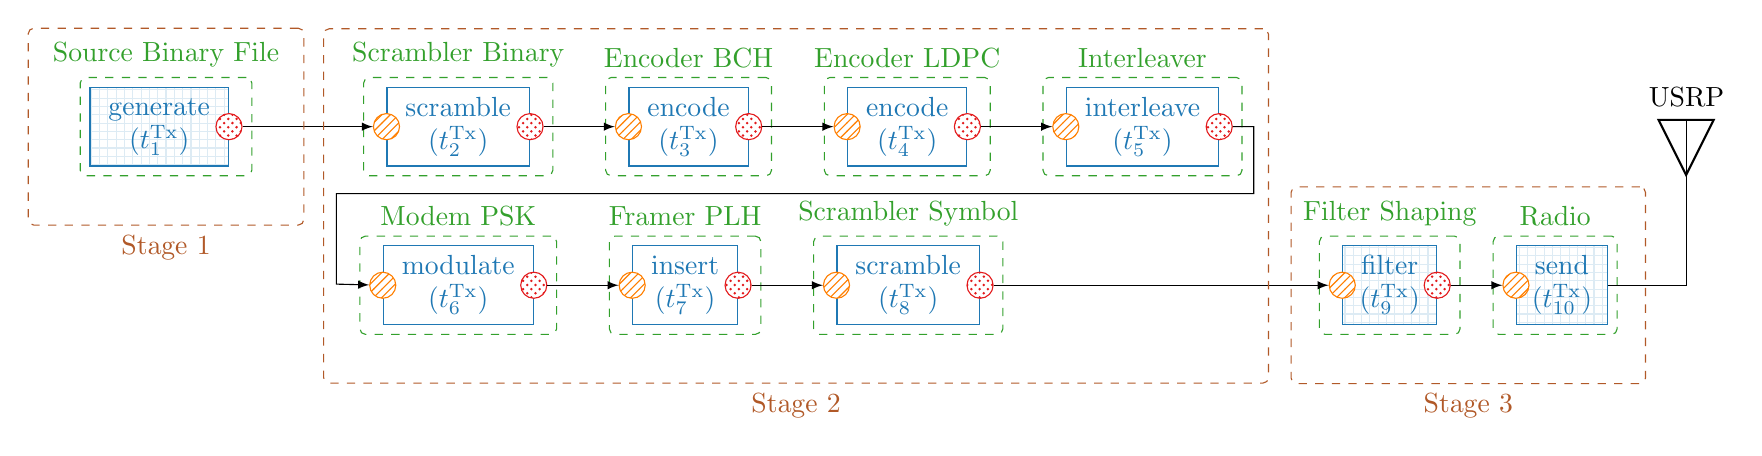
\begin{tikzpicture}%[scale=\tikzscale]
    \tikzset{ tsk/.style ={draw=Paired-1, rounded corners=0pt, text=Paired-1, minimum height=1.0cm, minimum width=1cm} }
    \tikzset{ stsk/.style={draw=Paired-1, rounded corners=0pt, text=Paired-1, minimum height=1.0cm, minimum width=1cm, preaction={fill=white}, pattern=grid, pattern color=Paired-1!15} }
    \tikzset{ ss/.style  ={draw=Paired-9, rounded corners=2pt, minimum height=1.5cm} }
    \tikzset{ seq/.style ={draw=Paired-11, dashed, rounded corners=2pt} }
    \tikzset{ mdl/.style ={draw=Paired-3,  dashed, rounded corners=2pt} }
    \tikzset{ pip/.style ={draw=Dark2-8,  dotted, thick, rounded corners=2pt} }
    \tikzset{ sin/.style ={draw=Paired-7, circle, minimum width=0.3cm, text=black, preaction={fill=white}, pattern=north east lines, pattern color=Paired-7} }
    \tikzset{ sout/.style={draw=Paired-5, circle, minimum width=0.3cm, text=black, preaction={fill=white}, pattern=crosshatch dots, pattern color=Paired-5} }

    \node[stsk                    , align=center] (t1) at (0.0, 2.0) {~generate~~\\($t^{\text{Tx}}_1$)};
    \node[tsk , right=2.00cm of t1, align=center] (t2)               {~scramble~~\\($t^{\text{Tx}}_2$)};
    \node[tsk , right=1.25cm of t2, align=center] (t3)               {~encode~~\\($t^{\text{Tx}}_3$)};
    \node[tsk , right=1.25cm of t3, align=center] (t4)               {~encode~~\\($t^{\text{Tx}}_4$)};
    \node[tsk , right=1.25cm of t4, align=center] (t5)               {~interleave~~\\($t^{\text{Tx}}_5$)};
    \node[tsk,  below=1.00cm of t2, align=center] (t6)               {~modulate~~\\($t^{\text{Tx}}_6$)};
    \node[tsk , right=1.25cm of t6, align=center] (t7)               {~insert~~\\($t^{\text{Tx}}_7$)};
    \node[tsk , right=1.25cm of t7, align=center] (t8)               {~scramble~~\\($t^{\text{Tx}}_8$)};
    \node[stsk, right=4.60cm of t8, align=center] (t9)               {~filter~~\\($t^{\text{Tx}}_9$)};
    \node[stsk, right=1.00cm of t9, align=center] (t10)              {~send~~\\($t^{\text{Tx}}_{10}$)};

    \node[sout, at=(t1.east) ] (t1_so)  {};
    \node[sin,  at=(t2.west) ] (t2_si)  {};
    \node[sout, at=(t2.east) ] (t2_so)  {};
    \node[sin,  at=(t3.west) ] (t3_si)  {};
    \node[sout, at=(t3.east) ] (t3_so)  {};
    \node[sin,  at=(t4.west) ] (t4_si)  {};
    \node[sout, at=(t4.east) ] (t4_so)  {};
    \node[sin,  at=(t5.west) ] (t5_si)  {};
    \node[sout, at=(t5.east) ] (t5_so)  {};
    \node[sin,  at=(t6.west) ] (t6_si)  {};
    \node[sout, at=(t6.east) ] (t6_so)  {};
    \node[sin,  at=(t7.west) ] (t7_si)  {};
    \node[sout, at=(t7.east) ] (t7_so)  {};
    \node[sin,  at=(t8.west) ] (t8_si)  {};
    \node[sout, at=(t8.east) ] (t8_so)  {};
    \node[sin,  at=(t9.west) ] (t9_si)  {};
    \node[sout, at=(t9.east) ] (t9_so)  {};
    \node[sin,  at=(t10.west)] (t10_si) {};

    \node[mdl, label={[Paired-3]above:Source Binary File},  fit=(t1)           (t1_so)] (m1) {};
    \node[mdl, label={[Paired-3]above:Scrambler Binary},    fit=(t2)  (t2_si)  (t2_so)] (m2) {};
    \node[mdl, label={[Paired-3]above:Encoder BCH},         fit=(t3)  (t3_si)  (t3_so)] (m3) {};
    \node[mdl, label={[Paired-3]above:Encoder LDPC},        fit=(t4)  (t4_si)  (t4_so)] (m4) {};
    \node[mdl, label={[Paired-3]above:Interleaver},         fit=(t5)  (t5_si)  (t5_so)] (m5) {};
    \node[mdl, label={[Paired-3]above:Modem PSK},           fit=(t6)  (t6_si)  (t6_so)] (m6) {};
    \node[mdl, label={[Paired-3]above:Framer PLH},          fit=(t7)  (t7_si)  (t7_so)] (m7) {};
    \node[mdl, label={[Paired-3]above:Scrambler Symbol},    fit=(t8)  (t8_si)  (t8_so)] (m8) {};
    \node[mdl, label={[Paired-3]above:Filter Shaping},      fit=(t9)  (t9_si)  (t9_so)] (m9) {};
    \node[mdl, label={[Paired-3]above:Radio},               fit=(t10) (t10_si)        ] (m9) {};

    \draw[->,>=latex] (t1_so) -- (t2_si)  node [midway, above] {};
    \draw[->,>=latex] (t2_so) -- (t3_si)  node [midway, above] {};
    \draw[->,>=latex] (t3_so) -- (t4_si)  node [midway, above] {};
    \draw[->,>=latex] (t4_so) -- (t5_si)  node [midway, above] {};
    \draw[->,>=latex] (t5_so) -- (13.9,2.0) -- (13.9,1.15) -- (2.25,1.15) -- (2.25,0) -- (t6_si)  node [midway, above] {};
    \draw[->,>=latex] (t6_so) -- (t7_si)  node [midway, above] {};
    \draw[->,>=latex] (t7_so) -- (t8_si)  node [midway, above] {};
    \draw[->,>=latex] (t8_so) -- (t9_si)  node [midway, above] {};
    \draw[->,>=latex] (t9_so) -- (t10_si) node [midway, above] {};
    \draw[black, -] (t10.east)--++(0:1.0cm) node[antenna, label={[above,yshift=+2.15cm]USRP}] {};

    \node[seq, minimum height=2.5cm, minimum width=3.5cm,  label={[Paired-11]below:Stage 1}, fit=(t1) (t1_so)                                      ] (seq1) {};
    \node[seq, minimum height=4.5cm, minimum width=12.0cm, label={[Paired-11]below:Stage 2}, fit=(t2_si) (t2) (t3) (t4) (t5) (t6) (t7) (t8) (t8_so)] (seq2) {};
    \node[seq, minimum height=2.5cm, minimum width=4.5cm,  label={[Paired-11]below:Stage 3}, fit=(t9_si) (t10)                                     ] (seq3) {};
  \end{tikzpicture}
\end{document}